%! Author = 207
%! Date = 2021/9/27

\part{研究背景和回顾}
    \chapter{研究背景}
        \section{研究起源}
        \section{问题描述}
        \section{研究意义}
    \chapter{现有的相关研究}
        \section{Literature Review(浓缩总结后)}
            \subsection{接触网络模型}
            \subsection{基于接触网络的传播模型}
            \subsection{防疫策略以及相关的评估标准}
        \section{阅读笔记(详细)}
            \subsection{传统的传播模型的文章阅读笔记}
            \subsection{基于Agent-based传播模型}
            \subsection{COVID-19病毒防控策略}
                COVID-19 病毒传播迅速,传染力极强,全球只有少量的国家能放置该病毒的传播,面对病毒的快速传播,不同的国家采取了不
                一样的检测措施,针对检测不同的检测对象可以分为三种方法\cite{crozier2021put}.
                \begin{itemize}
                    \item Symptomatic testing : Symptomatic testing检测策略仅对有症状的感染者进行检测,迅速对感染者追踪隔离,因此
                在检测率上往往有较高的准确率。目前使用该策略的国家有日本。
                    \item asymptomatic testing : asymptomatic testing 是一种针对无症状感染者的检测策略,这类方法目前是多数国家普遍采取的检测措施,并且不同的国家会针对不同的人群进行检测,英国和奥地利专注于定期检测保护易感染人群,
                    高风险地区。德国和比利时专注于对无症状感染者在5-7天进行每日检测,这类检测策略可以维持了成本和防疫力度的初步方法,对高
                    风险地区进行检测可以大大提高检测命中率,但是,随着时间的推移以及感染人数的增加,该方法的可行性还有待证明。
                    \item Mass testing: Mass testing大量的对社区的所有人群检测,或者对少量人口停止社区活动并进行重复性的检测。
                目前使用这类方法的有中国和越南,这类方法可以高效的控制病毒的传播,从而有效的抵御疫情,然而,这种方法成本极高,
                对于一些经济实力较弱的国家很难长期执行,一旦出现短时间内超级传播者经过多个地区进行全市甚至全省的检测,便需要极高的成本。
                \end{itemize}
                以上的三种方法在实际生活呈现出不同的状况。除了中国坚持Mass testing的方法使得整个国家仅有少数的个体感染外,其他的
                方法并没有。尽管Mass testing是真正意义上控制了感染人数的增长,然而这需要大量的劳动力成本和材料成本。
                因此,提高检测效率和降低成本扮演着控制病毒传播的关键地位,目前大量的研究针对经济和疫情的控制之间的平衡做出了相关的研究。

                [\cite{kolumbus2021effectiveness}] 提出了一个在多种高效干预措施下的SEIR的仿真模型,目的是权衡经济影响和健康之间的
                联系。在模型的模拟方面,作者模仿了现实情况,设置了一个E-R网络,每个节点的平均度为3.6(在没有任何干预
                下他引用别人的文章说是合理的),病人的平均潜伏期和平均感染期分别设置了6,8天,而感染率q = 0.5,
                病发概率为$p_{symp} = 1 - q^{1/8}$,总节点数10000,整个实验模型模拟了540天。在干预措施上
                作者在Lockdowns下按概率切断节点之间的边,也就是说,封锁程度0.3意味着存在连边的两个节点的边可能
                有30\%的概率会切断,针对隔离和追踪措施的干预下,对感染者的直接接触者进行检测,只隔离检测呈阳性的人。
                此外,作者使用封锁程度来衡量劳动力的损失情况,即考虑到的只是封锁程度与劳动力存在线性关系。
                结果表明,检测和隔离的结合能有效的减少经济经济成本呢死亡率,但是大量的检测有显著的效果。
                跟踪结合适度的测试能力可以在没有封锁的情况下实现遏制。(copy)
                跟踪和检测结合起来以降低死亡率和经济成本的政策极其有用,它们有可能在不施加任何社交距离限制的情况下遏制疫情。
                这突出了交易的棘手的社会问题——这些收益与病人的隐私相冲突,追踪不可避免地侵犯了病人的隐私。

                [\cite{eilersen2020cost}] 专注于衡量在有限的隔离与检测的情况下减缓成本收益 同样地使用SEIR仿真模型进行研究,但作者不仅将个体分为30\%Work,40\%Family,15\%Friends,15\%Public,
                而且在状态的持续时间有所调整,令S,I,R的状态平均维持在时间3天,从E到I的平均时间为5天,其中有一半的时间
                维持着E的状态,后半段时间维持Pre-symptomatic(infectious)的过度状态。在个体的设置上是模仿了丹麦的人口
                分布,平均每个个体有2位亲人,10位工友,两组朋友每组有5位。每个个体每一轮(0.5day)拥有一定概率抽到扮演着这4中
                角色的机会,总共5000个个体,最后感染率的设置是美国死亡率 + 23\%。结果表明,图\ref{fig:paper_result1}是实验的结果,
                减少工作、社交接触、减少工作间的规模程度能有效的延缓并降低感染人数。接着,作者使用 1 step tracing
                and quarantine strategy(1STQ)策略,即
                \begin{itemize}
                    \item close the workplaces of people who are tested positive for the disease.
                    \item isolate their regular social contacts for a limited period
                    \item keep symptomatic individuals in quarantine until they recover.
                \end{itemize}
                \begin{figure}[htbp]
                    \centering
                    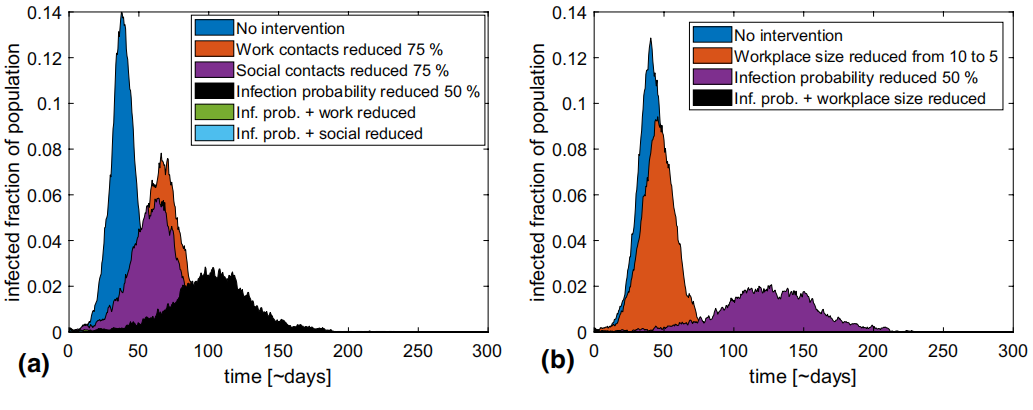
\includegraphics[scale = 0.5]{./img/paper/eilersen2020cost/1}
                    \label{fig:paper_result1}
                \end{figure}
                \begin{figure}[htbp]
                    \centering
                    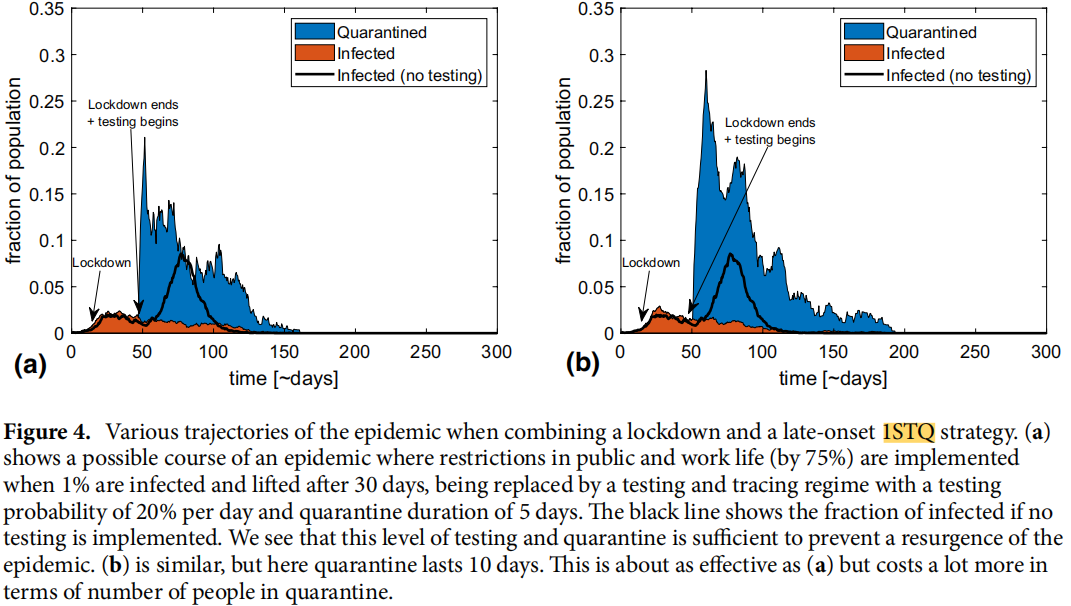
\includegraphics[scale = 0.3]{./img/paper/eilersen2020cost/2}
                    \label{fig:paper_result2}
                \end{figure}
                这种策略与overall Lockdown相比可以大大减少损失的工作日。如图\ref{fig:paper_result2}为采取封锁与未采取任何措施
                的结果,非常有意思的是,当Lockdown解除以后的30天开始检测隔离措施,隔离了大量的个体,最高甚至达到约
                30\%,而no testing 的感染人数尽管并没有隔离任由病毒在相同的环境下传播,但是最高的感染人数不过10\%,
                Quarantined 的节点是需要隔离5天的,无隔离措施的感染人数最高占约10\%,并持续时间大概在50天左右,而
                采取隔离措施的情况却是隔离人数最高甚至接近30\%,并持续约150天。我认为这样的隔离措施过于粗糙,假设
                病毒不会变异的情况下,尽管采取了这样的措施在50-100天的感染人数
                大大减少,隔离的人数和持续时间可以侧面反应成本,因此不难发现成本之大,也就是说尽管从结果上看采取1STQ的
                措施能大大减少损失的工作日,但是由于隔离的人数大大增加,损失了大量的劳动力。
        \section{针对前人的研究存在的问题提出的改进思路}
            \begin{figure}[htbp]
            \centering
            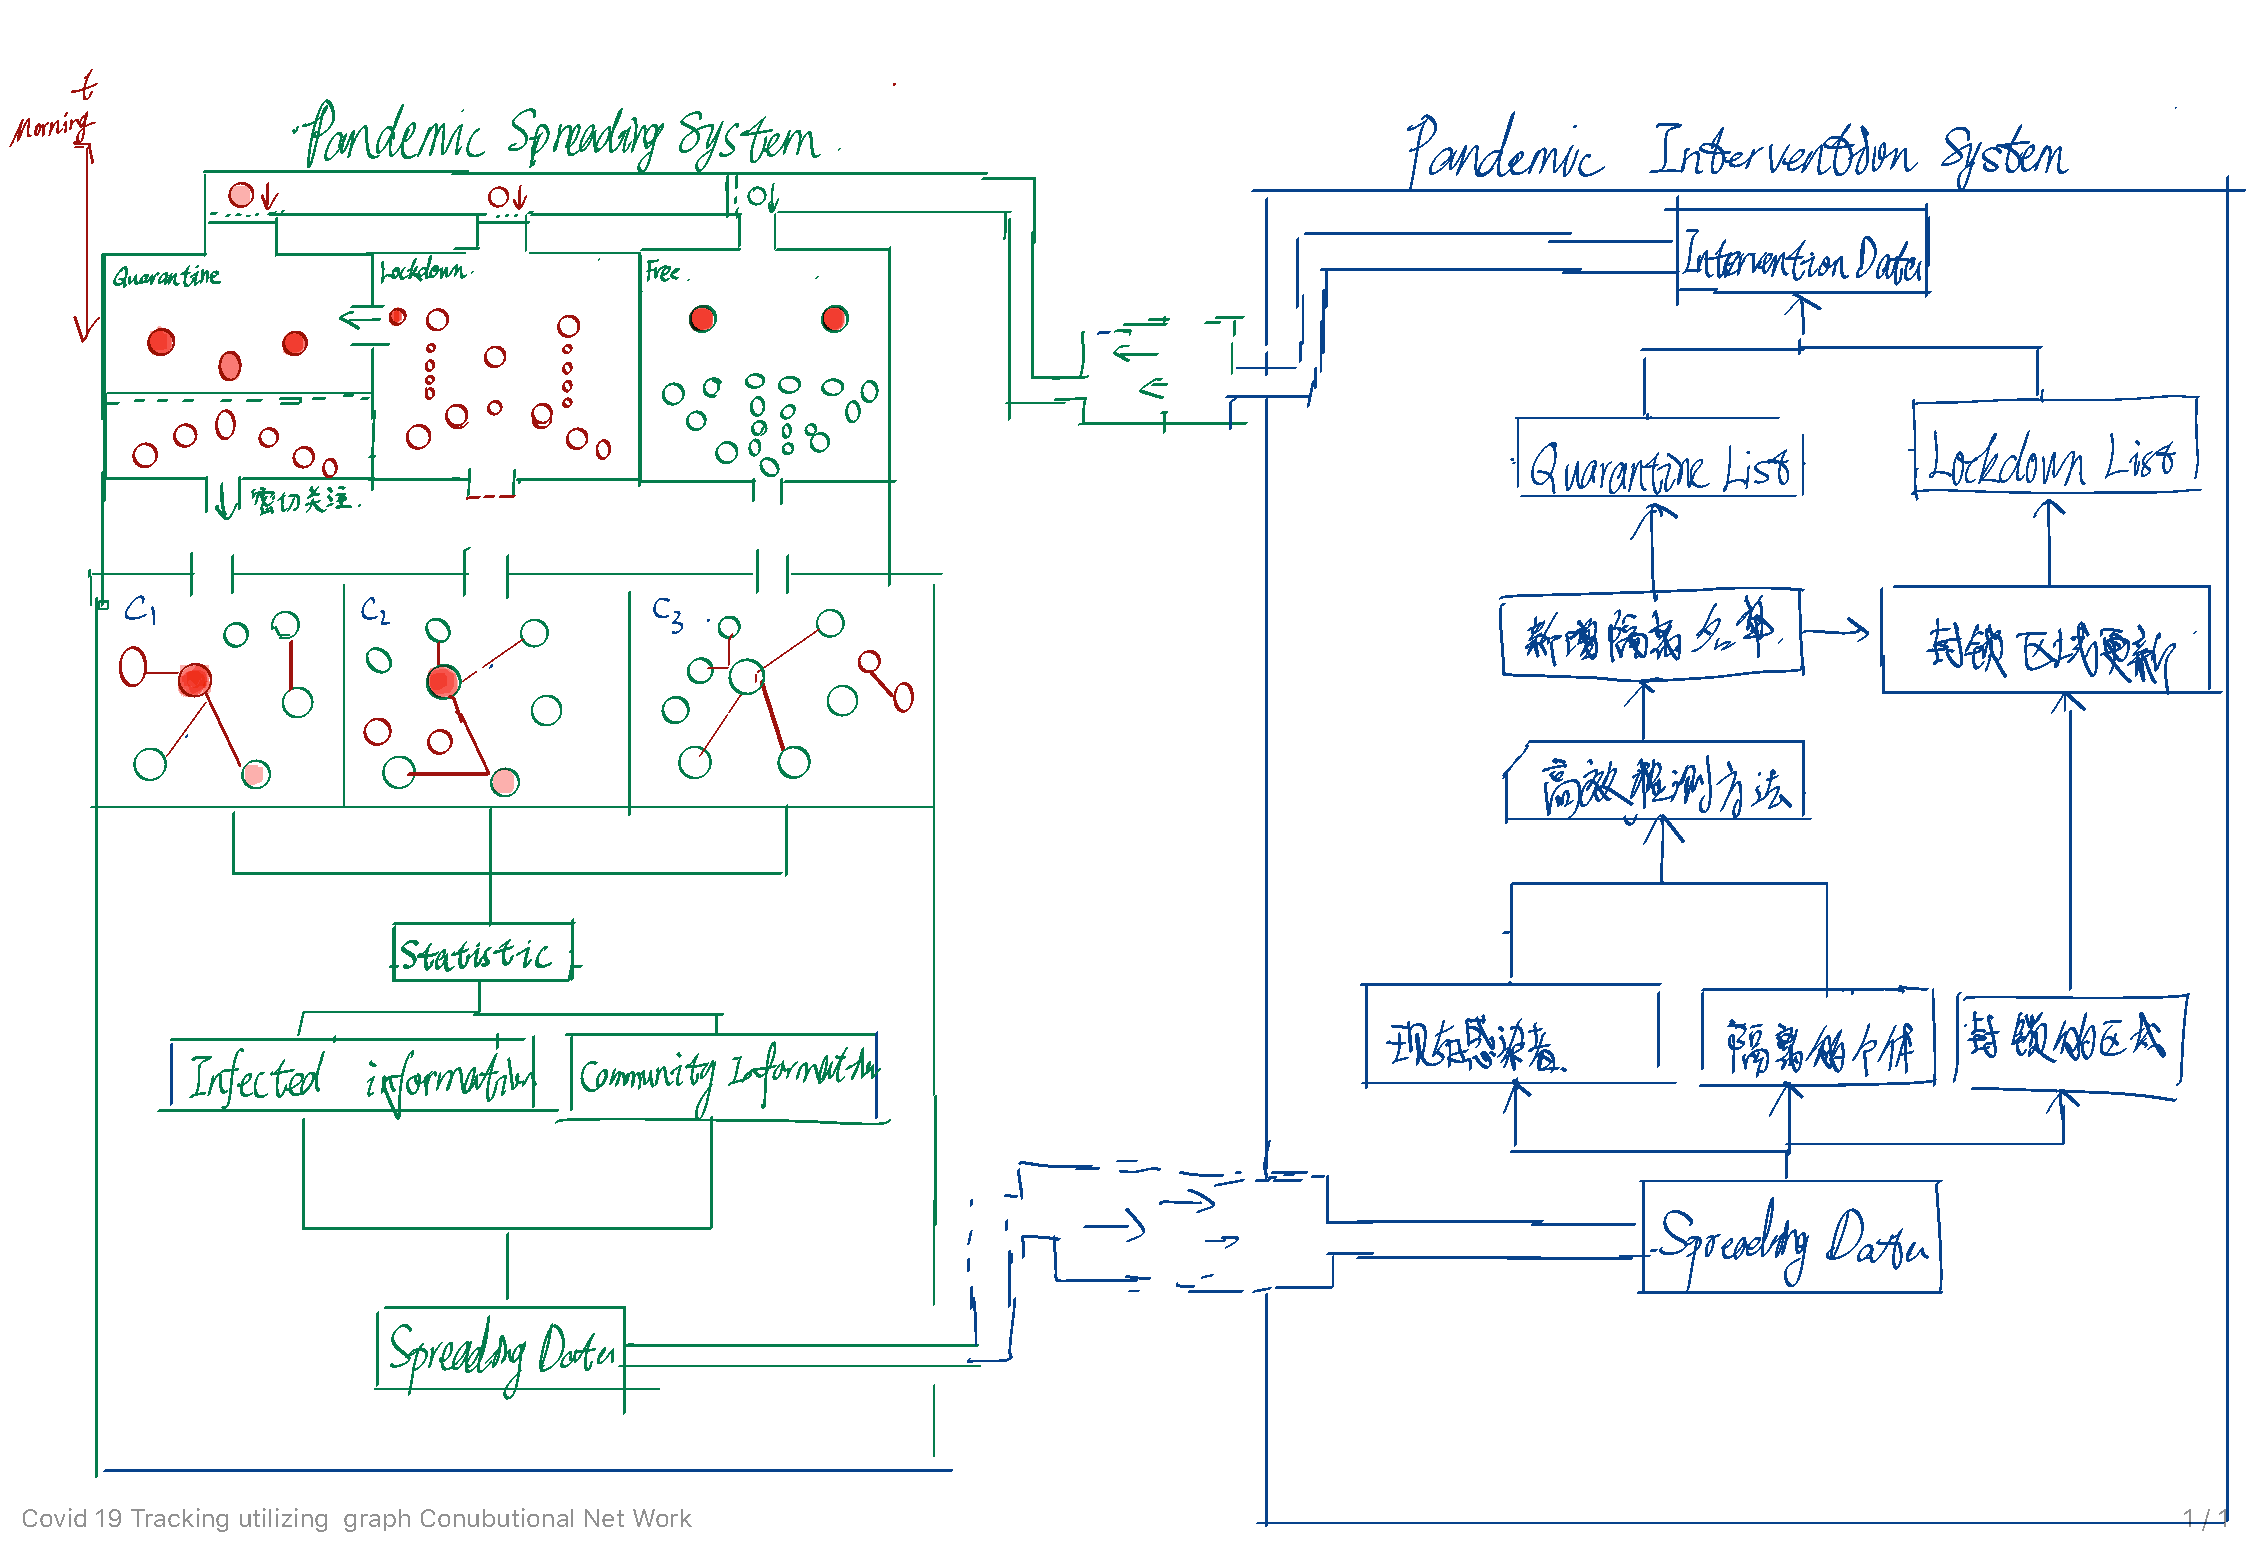
\includegraphics[scale = 0.40]{./img/workflow.pdf}
            \label{fig:workflow simulation}
            \caption{整个系统包括病毒传播系统(Pandemic Spreading System,PSS)和
            病毒干预措施系统(Pandemic Intervention System,PIS),在PSS中,红色的节点代表已确诊,红白的节点代表
            密切关注者,而绿白的节点代表易感人群和潜伏者。此外,流程图中设定了1个隔离区,1个封锁区,4个自由区作为示例。
            在隔离区,以虚实线分为必须隔离区和非必须隔离区,已确诊的节点隔离在必须隔离区,密切关注者则的行动与绿色的节点
            无差异,但必须采取戴口罩的措施,否则不能进入自由区。在自由区,节点可以根据偏好随意活动,
            只能跟同一区域内的节点接触。接着,每天统计感染者信息和所在的社区信息传输到PIS系统。收到了
            PSS传输的数据后,PIS根据现存的感染者和隔离的个体的状态信息,统计全部在自由区的有症状
            感染者所在的区域,对这些区域中所在的所有节点都进行检测并隔离,对于检测到为感染者的则安排到必须
            隔离区,而其他的节点则安排到非必须隔离区。接着,如果实行区域封锁,则将感染者所在区域进行全面封锁,
            除了已确诊的节点可以通往必须隔离区,封锁区域中的节点不能到其他的区域直到封锁期结束。}
        \end{figure}
